% Created by tikzDevice version 0.12 on 2018-09-28 04:16:17
% !TEX encoding = UTF-8 Unicode
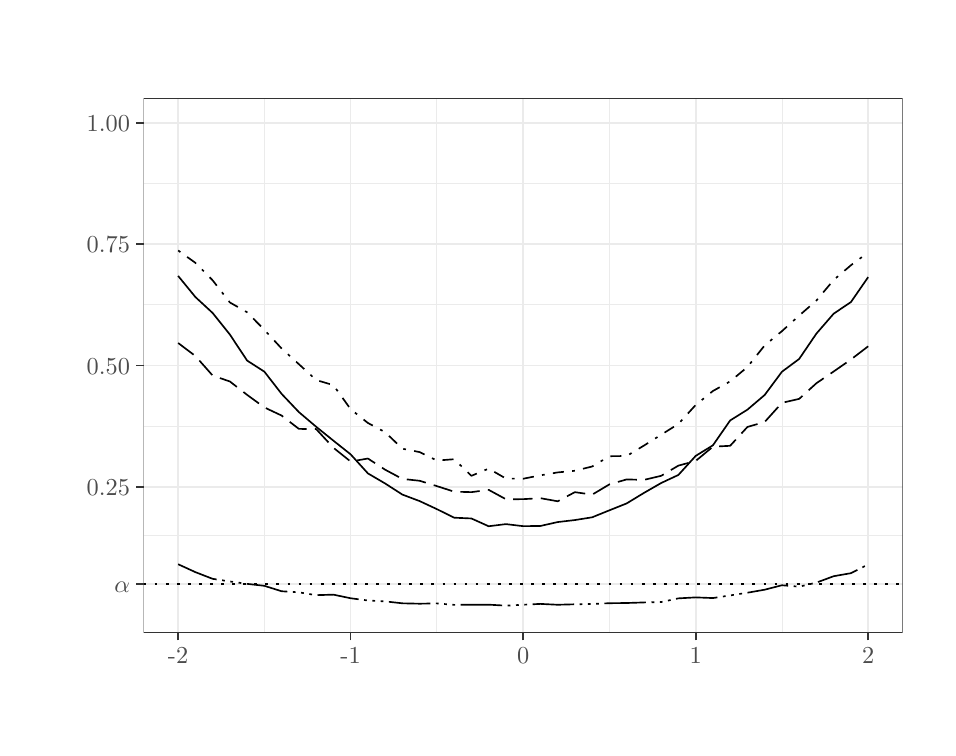
\begin{tikzpicture}[x=1pt,y=1pt]
\definecolor{fillColor}{RGB}{255,255,255}
\path[use as bounding box,fill=fillColor,fill opacity=0.00] (0,0) rectangle (325.21,252.94);
\begin{scope}
\path[clip] (  0.00,  0.00) rectangle (325.21,252.94);
\definecolor{drawColor}{RGB}{255,255,255}
\definecolor{fillColor}{RGB}{255,255,255}

\path[draw=drawColor,line width= 0.6pt,line join=round,line cap=round,fill=fillColor] (  0.00,  0.00) rectangle (325.21,252.94);
\end{scope}
\begin{scope}
\path[clip] ( 41.90, 34.26) rectangle (316.18,227.38);
\definecolor{fillColor}{RGB}{255,255,255}

\path[fill=fillColor] ( 41.90, 34.26) rectangle (316.18,227.38);
\definecolor{drawColor}{gray}{0.92}

\path[draw=drawColor,line width= 0.3pt,line join=round] ( 41.90, 69.37) --
	(316.18, 69.37);

\path[draw=drawColor,line width= 0.3pt,line join=round] ( 41.90,108.87) --
	(316.18,108.87);

\path[draw=drawColor,line width= 0.3pt,line join=round] ( 41.90,152.76) --
	(316.18,152.76);

\path[draw=drawColor,line width= 0.3pt,line join=round] ( 41.90,196.65) --
	(316.18,196.65);

\path[draw=drawColor,line width= 0.3pt,line join=round] ( 85.53, 34.26) --
	( 85.53,227.38);

\path[draw=drawColor,line width= 0.3pt,line join=round] (147.87, 34.26) --
	(147.87,227.38);

\path[draw=drawColor,line width= 0.3pt,line join=round] (210.21, 34.26) --
	(210.21,227.38);

\path[draw=drawColor,line width= 0.3pt,line join=round] (272.55, 34.26) --
	(272.55,227.38);

\path[draw=drawColor,line width= 0.6pt,line join=round] ( 41.90, 51.81) --
	(316.18, 51.81);

\path[draw=drawColor,line width= 0.6pt,line join=round] ( 41.90, 86.93) --
	(316.18, 86.93);

\path[draw=drawColor,line width= 0.6pt,line join=round] ( 41.90,130.82) --
	(316.18,130.82);

\path[draw=drawColor,line width= 0.6pt,line join=round] ( 41.90,174.71) --
	(316.18,174.71);

\path[draw=drawColor,line width= 0.6pt,line join=round] ( 41.90,218.60) --
	(316.18,218.60);

\path[draw=drawColor,line width= 0.6pt,line join=round] ( 54.37, 34.26) --
	( 54.37,227.38);

\path[draw=drawColor,line width= 0.6pt,line join=round] (116.70, 34.26) --
	(116.70,227.38);

\path[draw=drawColor,line width= 0.6pt,line join=round] (179.04, 34.26) --
	(179.04,227.38);

\path[draw=drawColor,line width= 0.6pt,line join=round] (241.38, 34.26) --
	(241.38,227.38);

\path[draw=drawColor,line width= 0.6pt,line join=round] (303.71, 34.26) --
	(303.71,227.38);
\definecolor{drawColor}{RGB}{0,0,0}

\path[draw=drawColor,line width= 0.6pt,dash pattern=on 1pt off 3pt on 4pt off 3pt ,line join=round] ( 54.37,172.43) --
	( 60.60,167.97) --
	( 66.83,161.65) --
	( 73.07,153.64) --
	( 79.30,150.09) --
	( 85.53,143.74) --
	( 91.77,137.00) --
	( 98.00,131.34) --
	(104.24,125.62) --
	(110.47,123.76) --
	(116.70,115.09) --
	(122.94,110.10) --
	(129.17,106.77) --
	(135.40,100.80) --
	(141.64, 99.57) --
	(147.87, 96.51) --
	(154.10, 97.00) --
	(160.34, 91.00) --
	(166.57, 93.60) --
	(172.81, 90.02) --
	(179.04, 89.95) --
	(185.27, 91.18) --
	(191.51, 92.23) --
	(197.74, 92.83) --
	(203.97, 94.37) --
	(210.21, 98.09) --
	(216.44, 98.16) --
	(222.68,101.92) --
	(228.91,105.85) --
	(235.14,109.75) --
	(241.38,116.60) --
	(247.61,121.65) --
	(253.84,125.13) --
	(260.08,130.33) --
	(266.31,138.12) --
	(272.55,143.28) --
	(278.78,148.90) --
	(285.01,154.34) --
	(291.25,161.79) --
	(297.48,167.09) --
	(303.71,171.72);

\path[draw=drawColor,line width= 0.6pt,dash pattern=on 15pt off 2pt on 1pt off 2pt on 1pt off 2pt on 1pt off 2pt ,line join=round] ( 54.37, 59.05) --
	( 60.60, 56.20) --
	( 66.83, 53.78) --
	( 73.07, 52.83) --
	( 79.30, 51.96) --
	( 85.53, 51.25) --
	( 91.77, 49.29) --
	( 98.00, 48.90) --
	(104.24, 47.88) --
	(110.47, 48.06) --
	(116.70, 46.76) --
	(122.94, 45.95) --
	(129.17, 45.63) --
	(135.40, 44.93) --
	(141.64, 44.79) --
	(147.87, 44.90) --
	(154.10, 44.37) --
	(160.34, 44.44) --
	(166.57, 44.44) --
	(172.81, 44.09) --
	(179.04, 44.41) --
	(185.27, 44.72) --
	(191.51, 44.41) --
	(197.74, 44.58) --
	(203.97, 44.69) --
	(210.21, 44.97) --
	(216.44, 45.04) --
	(222.68, 45.25) --
	(228.91, 45.39) --
	(235.14, 46.72) --
	(241.38, 47.07) --
	(247.61, 46.83) --
	(253.84, 47.78) --
	(260.08, 48.76) --
	(266.31, 49.85) --
	(272.55, 51.46) --
	(278.78, 50.94) --
	(285.01, 52.41) --
	(291.25, 54.73) --
	(297.48, 55.82) --
	(303.71, 58.98);

\path[draw=drawColor,line width= 0.6pt,dash pattern=on 7pt off 3pt ,line join=round] ( 54.37,139.00) --
	( 60.60,134.29) --
	( 66.83,127.24) --
	( 73.07,125.09) --
	( 79.30,120.25) --
	( 85.53,115.72) --
	( 91.77,112.77) --
	( 98.00,107.96) --
	(104.24,107.89) --
	(110.47,101.15) --
	(116.70, 96.16) --
	(122.94, 97.25) --
	(129.17, 93.21) --
	(135.40, 89.88) --
	(141.64, 89.21) --
	(147.87, 87.28) --
	(154.10, 85.28) --
	(160.34, 85.10) --
	(166.57, 85.94) --
	(172.81, 82.54) --
	(179.04, 82.57) --
	(185.27, 82.92) --
	(191.51, 81.80) --
	(197.74, 85.10) --
	(203.97, 84.19) --
	(210.21, 87.91) --
	(216.44, 89.70) --
	(222.68, 89.53) --
	(228.91, 91.00) --
	(235.14, 94.69) --
	(241.38, 96.37) --
	(247.61,101.53) --
	(253.84,101.85) --
	(260.08,108.66) --
	(266.31,110.45) --
	(272.55,117.37) --
	(278.78,118.81) --
	(285.01,124.46) --
	(291.25,128.71) --
	(297.48,133.03) --
	(303.71,137.80);

\path[draw=drawColor,line width= 0.6pt,line join=round] ( 54.37,163.23) --
	( 60.60,155.61) --
	( 66.83,149.85) --
	( 73.07,142.05) --
	( 79.30,132.64) --
	( 85.53,128.64) --
	( 91.77,120.60) --
	( 98.00,114.03) --
	(104.24,108.73) --
	(110.47,103.71) --
	(116.70, 98.76) --
	(122.94, 91.88) --
	(129.17, 88.23) --
	(135.40, 84.22) --
	(141.64, 81.87) --
	(147.87, 78.96) --
	(154.10, 75.87) --
	(160.34, 75.59) --
	(166.57, 72.78) --
	(172.81, 73.55) --
	(179.04, 72.81) --
	(185.27, 72.88) --
	(191.51, 74.29) --
	(197.74, 75.02) --
	(203.97, 76.01) --
	(210.21, 78.54) --
	(216.44, 81.03) --
	(222.68, 84.82) --
	(228.91, 88.40) --
	(235.14, 91.32) --
	(241.38, 98.20) --
	(247.61,102.03) --
	(253.84,111.01) --
	(260.08,114.91) --
	(266.31,120.21) --
	(272.55,128.61) --
	(278.78,133.24) --
	(285.01,142.40) --
	(291.25,149.60) --
	(297.48,153.78) --
	(303.71,162.80);

\path[draw=drawColor,line width= 0.6pt,dash pattern=on 1pt off 3pt ,line join=round] ( 41.90, 51.81) -- (316.18, 51.81);
\definecolor{drawColor}{gray}{0.20}

\path[draw=drawColor,line width= 0.6pt,line join=round,line cap=round] ( 41.90, 34.26) rectangle (316.18,227.38);
\end{scope}
\begin{scope}
\path[clip] (  0.00,  0.00) rectangle (325.21,252.94);
\definecolor{drawColor}{gray}{0.30}

\node[text=drawColor,anchor=base east,inner sep=0pt, outer sep=0pt, scale=  0.88] at ( 36.95, 48.78) {$\alpha$};

\node[text=drawColor,anchor=base east,inner sep=0pt, outer sep=0pt, scale=  0.88] at ( 36.95, 83.90) {$0.25$};

\node[text=drawColor,anchor=base east,inner sep=0pt, outer sep=0pt, scale=  0.88] at ( 36.95,127.79) {$0.50$};

\node[text=drawColor,anchor=base east,inner sep=0pt, outer sep=0pt, scale=  0.88] at ( 36.95,171.68) {$0.75$};

\node[text=drawColor,anchor=base east,inner sep=0pt, outer sep=0pt, scale=  0.88] at ( 36.95,215.57) {$1.00$};
\end{scope}
\begin{scope}
\path[clip] (  0.00,  0.00) rectangle (325.21,252.94);
\definecolor{drawColor}{gray}{0.20}

\path[draw=drawColor,line width= 0.6pt,line join=round] ( 39.15, 51.81) --
	( 41.90, 51.81);

\path[draw=drawColor,line width= 0.6pt,line join=round] ( 39.15, 86.93) --
	( 41.90, 86.93);

\path[draw=drawColor,line width= 0.6pt,line join=round] ( 39.15,130.82) --
	( 41.90,130.82);

\path[draw=drawColor,line width= 0.6pt,line join=round] ( 39.15,174.71) --
	( 41.90,174.71);

\path[draw=drawColor,line width= 0.6pt,line join=round] ( 39.15,218.60) --
	( 41.90,218.60);
\end{scope}
\begin{scope}
\path[clip] (  0.00,  0.00) rectangle (325.21,252.94);
\definecolor{drawColor}{gray}{0.20}

\path[draw=drawColor,line width= 0.6pt,line join=round] ( 54.37, 31.51) --
	( 54.37, 34.26);

\path[draw=drawColor,line width= 0.6pt,line join=round] (116.70, 31.51) --
	(116.70, 34.26);

\path[draw=drawColor,line width= 0.6pt,line join=round] (179.04, 31.51) --
	(179.04, 34.26);

\path[draw=drawColor,line width= 0.6pt,line join=round] (241.38, 31.51) --
	(241.38, 34.26);

\path[draw=drawColor,line width= 0.6pt,line join=round] (303.71, 31.51) --
	(303.71, 34.26);
\end{scope}
\begin{scope}
\path[clip] (  0.00,  0.00) rectangle (325.21,252.94);
\definecolor{drawColor}{gray}{0.30}

\node[text=drawColor,anchor=base,inner sep=0pt, outer sep=0pt, scale=  0.88] at ( 54.37, 23.25) {-2};

\node[text=drawColor,anchor=base,inner sep=0pt, outer sep=0pt, scale=  0.88] at (116.70, 23.25) {-1};

\node[text=drawColor,anchor=base,inner sep=0pt, outer sep=0pt, scale=  0.88] at (179.04, 23.25) {0};

\node[text=drawColor,anchor=base,inner sep=0pt, outer sep=0pt, scale=  0.88] at (241.38, 23.25) {1};

\node[text=drawColor,anchor=base,inner sep=0pt, outer sep=0pt, scale=  0.88] at (303.71, 23.25) {2};
\end{scope}
\end{tikzpicture}
